\subsection{The Challenges: Foregrounds, systematics}
\label{sec:foregrounds}
\vspace{-0.05in}
\comred{3 pages. Discuss the challenge of Foregrounds and Systematics. }

\begin{figure}[h]
\begin{center}
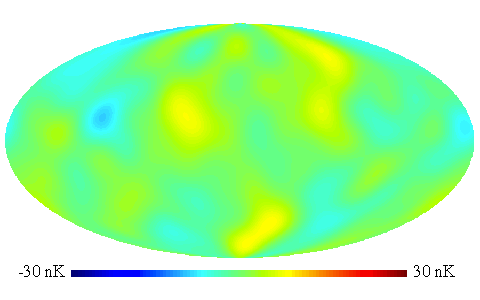
\includegraphics[width=3.2in]{Figures/P15_2_12_rp001.pdf}
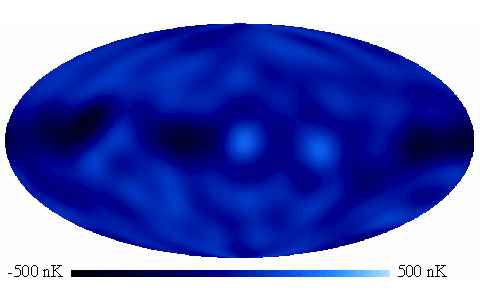
\includegraphics[width=3.2in]{Figures/P353_N_2_12.pdf}
\end{center}
\caption{}
\label{fig:qrp001}
\end{figure}

\begin{figure}[h]
\begin{center}
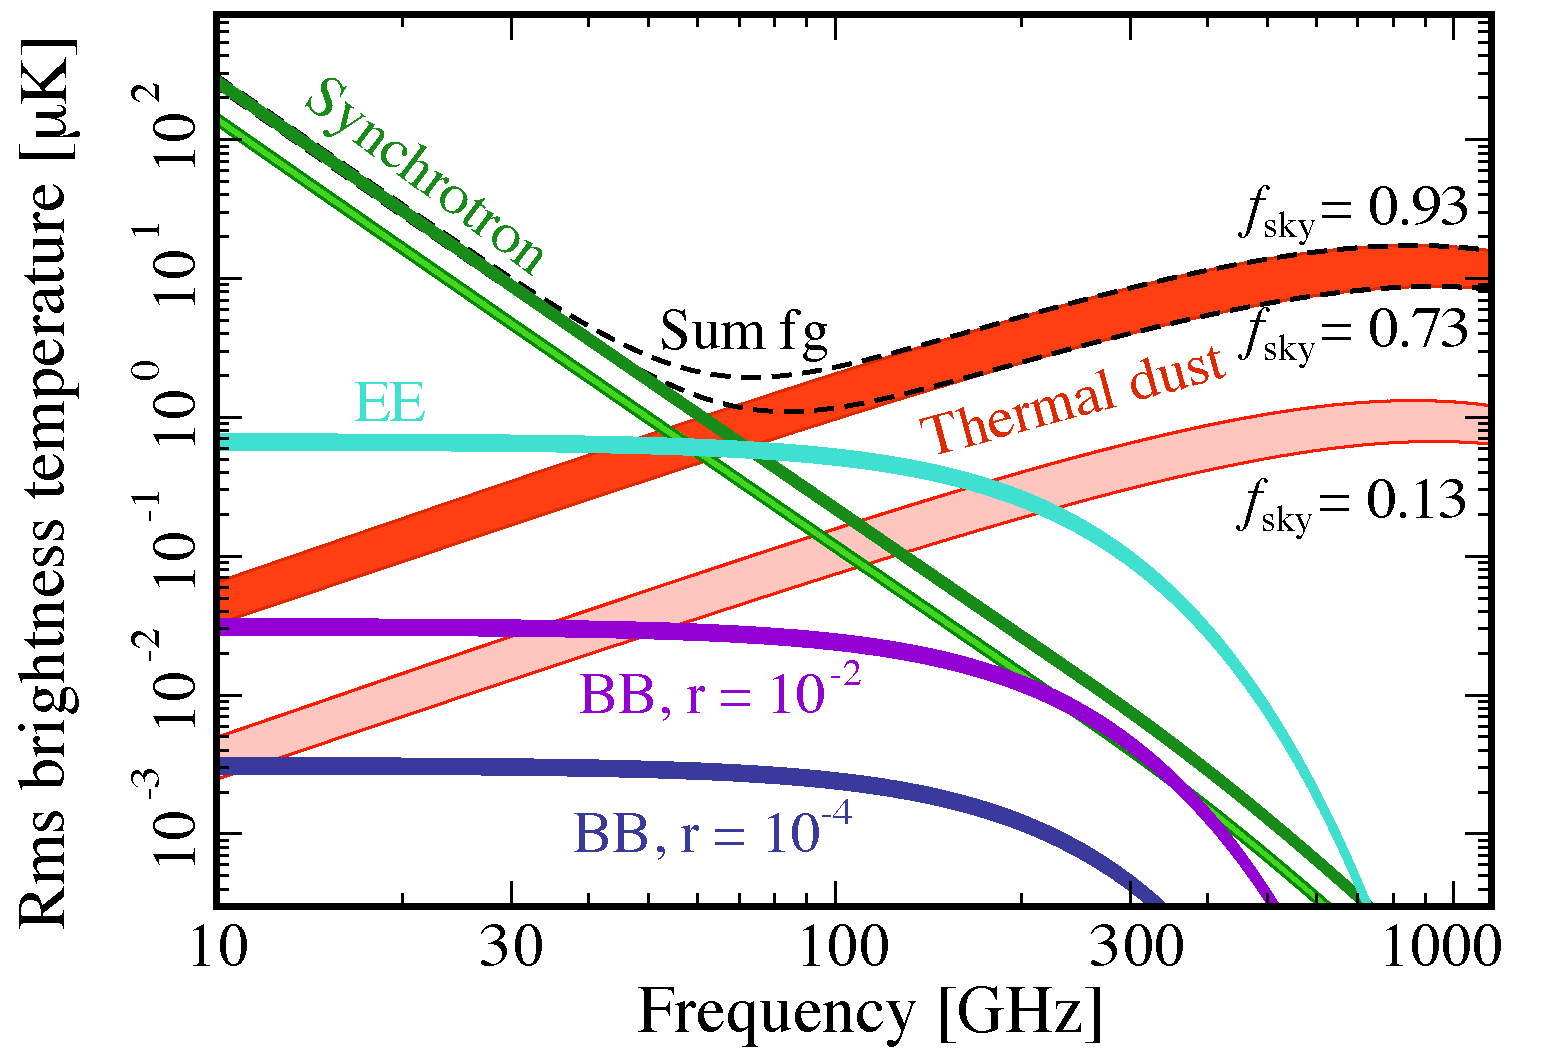
\includegraphics[width=3.26in]{Figures/overview_pol_v4_fsky_noplanck.pdf}\hskip .2cm
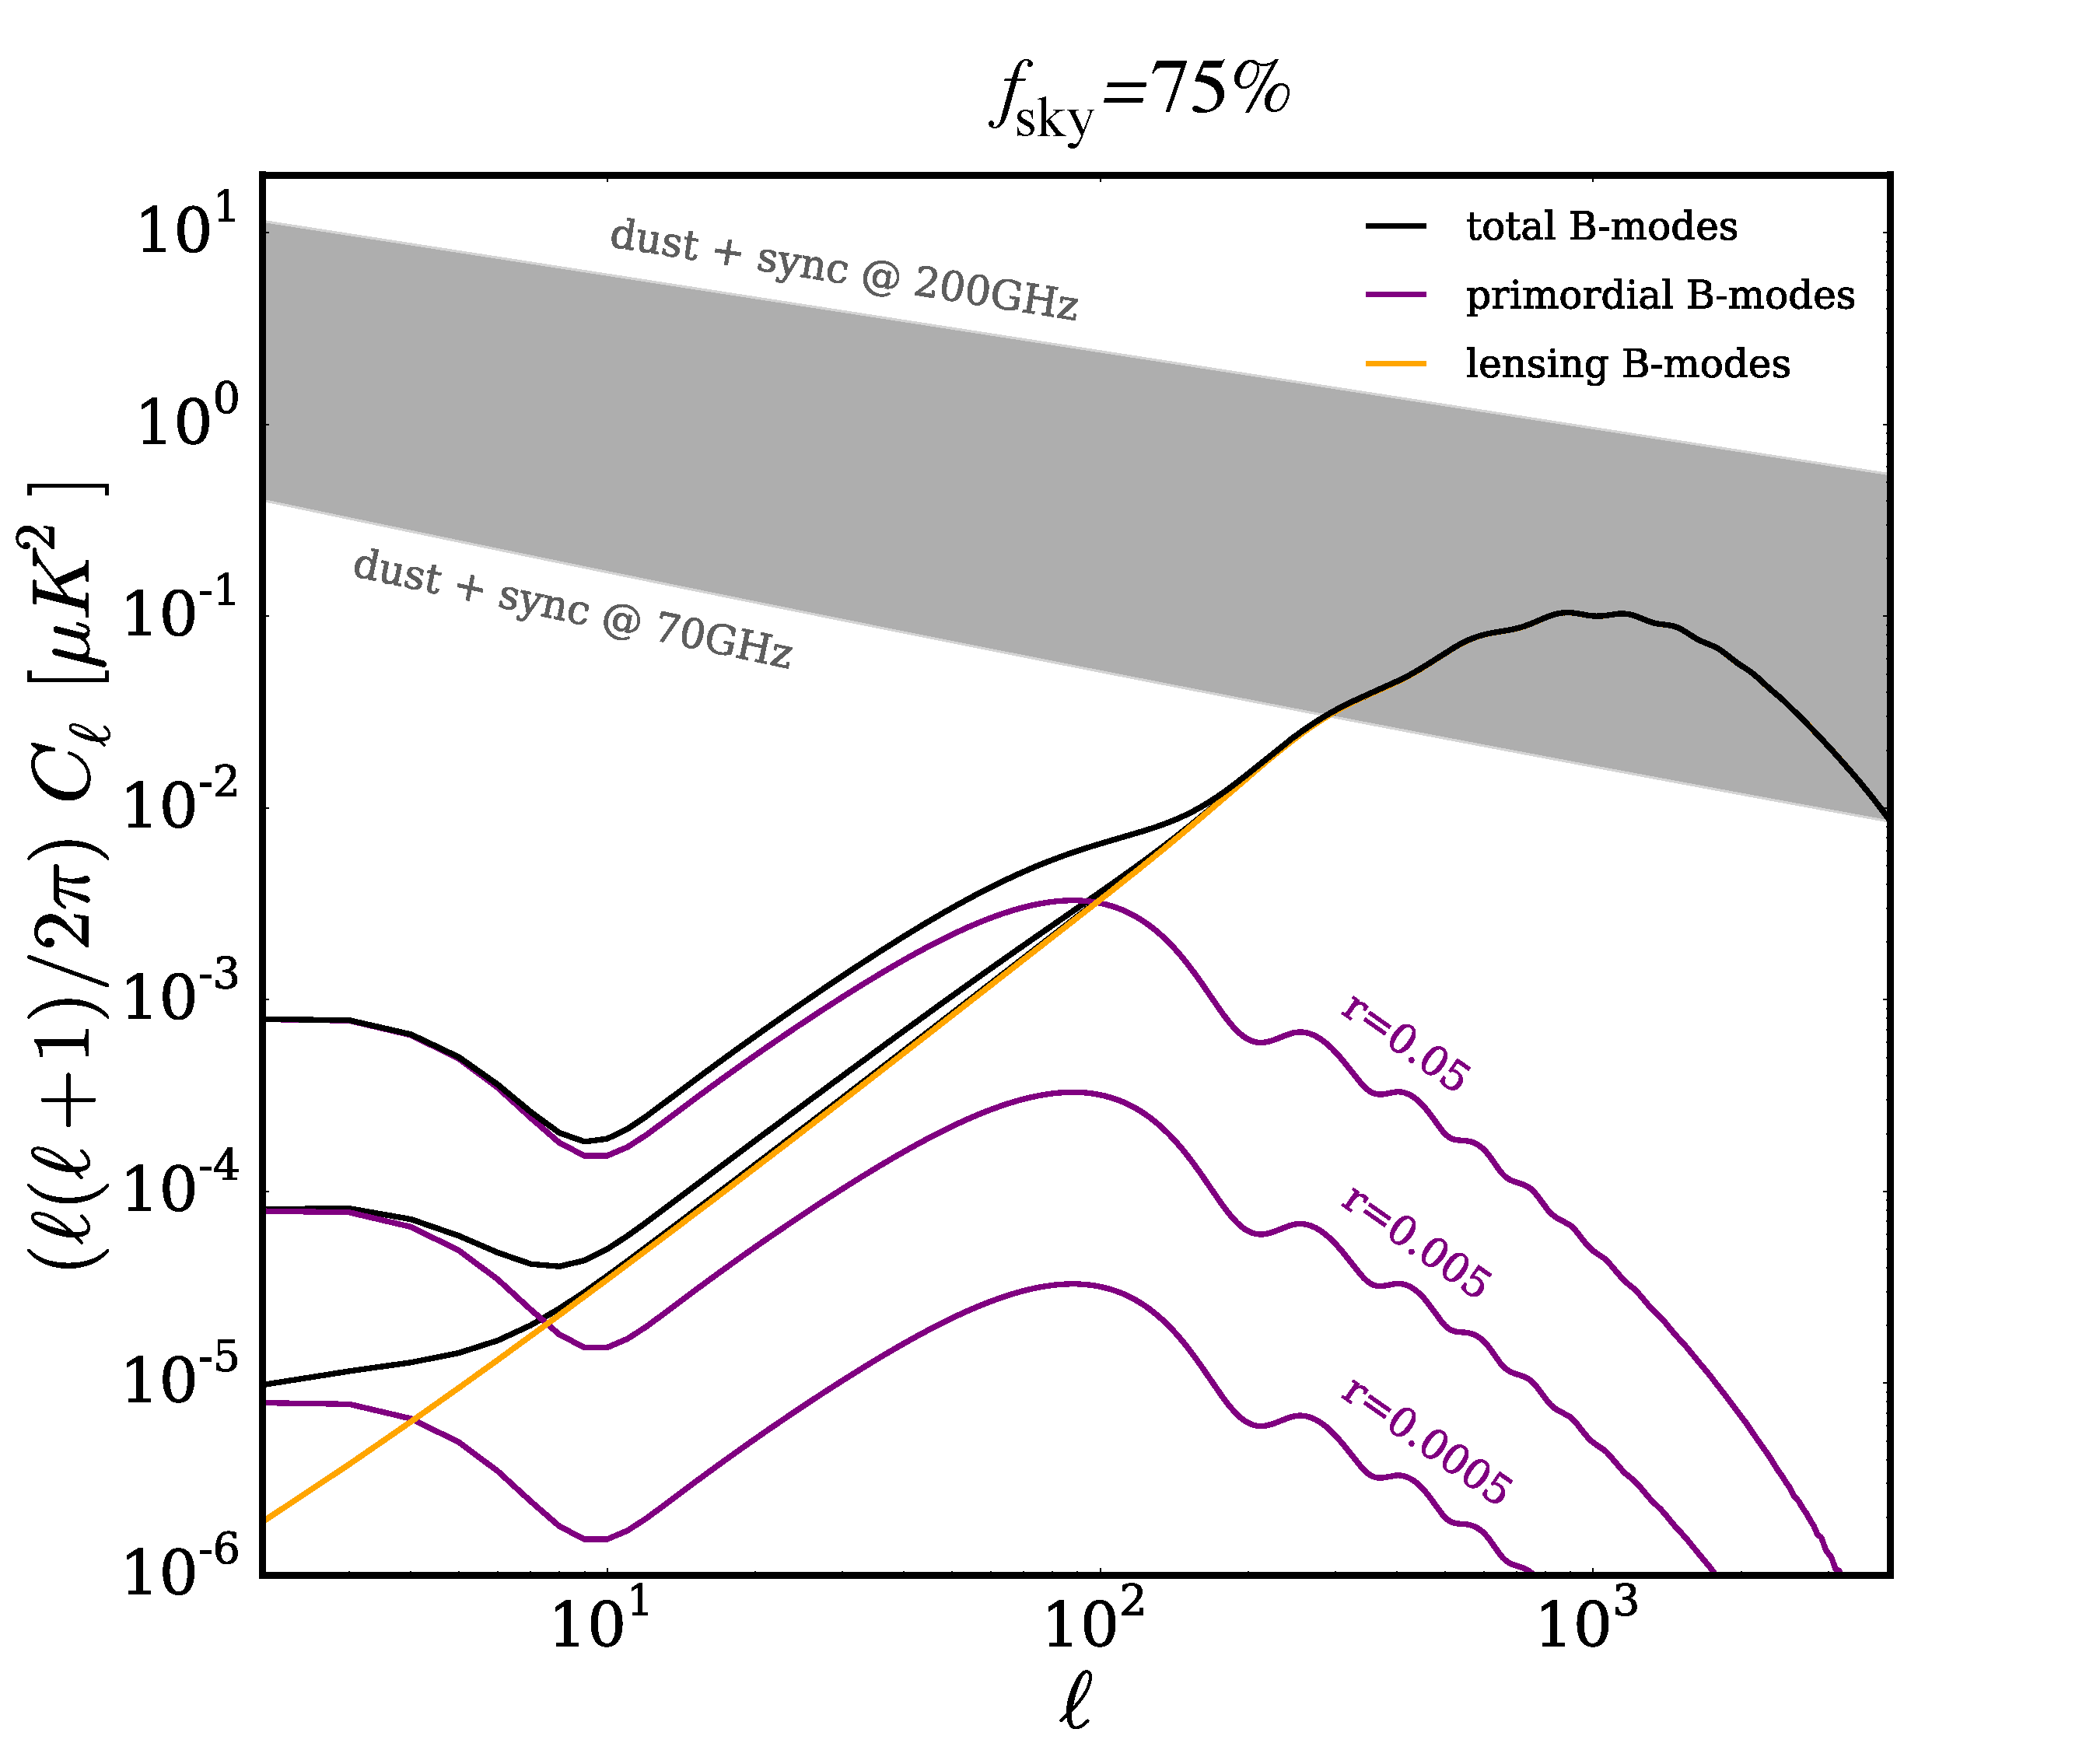
\includegraphics[width=3.12in]{Figures/clbb_freq.pdf}
\end{center}
\caption{}
\label{fig:frequency}
\end{figure}

\subsubsection{Systematic Effects}
\label{sec:systematics}
\begin{itemize}
\item Intensity-to-polarization leakage: Differential pointing,
  differential beams, gain errors, bandpass mismatch leakage 
\item Stability: Thermal drifts, space radiation environment
\item Straylight: polarized far-sidelobe pickup
\end{itemize}

% Raphael, Josquin, Aurelien, Charles
